\documentclass[twoside]{book}

% Packages required by doxygen
\usepackage{fixltx2e}
\usepackage{calc}
\usepackage{doxygen}
\usepackage{graphicx}
\usepackage[utf8]{inputenc}
\usepackage{makeidx}
\usepackage{multicol}
\usepackage{multirow}
\PassOptionsToPackage{warn}{textcomp}
\usepackage{textcomp}
\usepackage[nointegrals]{wasysym}
\usepackage[table]{xcolor}

% Font selection
\usepackage[T1]{fontenc}
\usepackage{mathptmx}
\usepackage[scaled=.90]{helvet}
\usepackage{courier}
\usepackage{amssymb}
\usepackage{sectsty}
\renewcommand{\familydefault}{\sfdefault}
\allsectionsfont{%
  \fontseries{bc}\selectfont%
  \color{darkgray}%
}
\renewcommand{\DoxyLabelFont}{%
  \fontseries{bc}\selectfont%
  \color{darkgray}%
}
\newcommand{\+}{\discretionary{\mbox{\scriptsize$\hookleftarrow$}}{}{}}

% Page & text layout
\usepackage{geometry}
\geometry{%
  a4paper,%
  top=2.5cm,%
  bottom=2.5cm,%
  left=2.5cm,%
  right=2.5cm%
}
\tolerance=750
\hfuzz=15pt
\hbadness=750
\setlength{\emergencystretch}{15pt}
\setlength{\parindent}{0cm}
\setlength{\parskip}{0.2cm}
\makeatletter
\renewcommand{\paragraph}{%
  \@startsection{paragraph}{4}{0ex}{-1.0ex}{1.0ex}{%
    \normalfont\normalsize\bfseries\SS@parafont%
  }%
}
\renewcommand{\subparagraph}{%
  \@startsection{subparagraph}{5}{0ex}{-1.0ex}{1.0ex}{%
    \normalfont\normalsize\bfseries\SS@subparafont%
  }%
}
\makeatother

% Headers & footers
\usepackage{fancyhdr}
\pagestyle{fancyplain}
\fancyhead[LE]{\fancyplain{}{\bfseries\thepage}}
\fancyhead[CE]{\fancyplain{}{}}
\fancyhead[RE]{\fancyplain{}{\bfseries\leftmark}}
\fancyhead[LO]{\fancyplain{}{\bfseries\rightmark}}
\fancyhead[CO]{\fancyplain{}{}}
\fancyhead[RO]{\fancyplain{}{\bfseries\thepage}}
\fancyfoot[LE]{\fancyplain{}{}}
\fancyfoot[CE]{\fancyplain{}{}}
\fancyfoot[RE]{\fancyplain{}{\bfseries\scriptsize Generated on Wed Oct 15 2014 15\+:01\+:28 for My Project by Doxygen }}
\fancyfoot[LO]{\fancyplain{}{\bfseries\scriptsize Generated on Wed Oct 15 2014 15\+:01\+:28 for My Project by Doxygen }}
\fancyfoot[CO]{\fancyplain{}{}}
\fancyfoot[RO]{\fancyplain{}{}}
\renewcommand{\footrulewidth}{0.4pt}
\renewcommand{\chaptermark}[1]{%
  \markboth{#1}{}%
}
\renewcommand{\sectionmark}[1]{%
  \markright{\thesection\ #1}%
}

% Indices & bibliography
\usepackage{natbib}
\usepackage[titles]{tocloft}
\setcounter{tocdepth}{3}
\setcounter{secnumdepth}{5}
\makeindex

% Hyperlinks (required, but should be loaded last)
\usepackage{ifpdf}
\ifpdf
  \usepackage[pdftex,pagebackref=true]{hyperref}
\else
  \usepackage[ps2pdf,pagebackref=true]{hyperref}
\fi
\hypersetup{%
  colorlinks=true,%
  linkcolor=blue,%
  citecolor=blue,%
  unicode%
}

% Custom commands
\newcommand{\clearemptydoublepage}{%
  \newpage{\pagestyle{empty}\cleardoublepage}%
}


%===== C O N T E N T S =====

\begin{document}

% Titlepage & ToC
\hypersetup{pageanchor=false,
             bookmarks=true,
             bookmarksnumbered=true,
             pdfencoding=unicode
            }
\pagenumbering{roman}
\begin{titlepage}
\vspace*{7cm}
\begin{center}%
{\Large My Project }\\
\vspace*{1cm}
{\large Generated by Doxygen 1.8.8}\\
\vspace*{0.5cm}
{\small Wed Oct 15 2014 15:01:28}\\
\end{center}
\end{titlepage}
\clearemptydoublepage
\tableofcontents
\clearemptydoublepage
\pagenumbering{arabic}
\hypersetup{pageanchor=true}

%--- Begin generated contents ---
\chapter{Namespace Index}
\section{Namespace List}
Here is a list of all documented namespaces with brief descriptions\+:\begin{DoxyCompactList}
\item\contentsline{section}{\hyperlink{namespaceH__Driver__CORE}{H\+\_\+\+Driver\+\_\+\+C\+O\+R\+E} }{\pageref{namespaceH__Driver__CORE}}{}
\end{DoxyCompactList}

\chapter{Hierarchical Index}
\section{Class Hierarchy}
This inheritance list is sorted roughly, but not completely, alphabetically\+:\begin{DoxyCompactList}
\item \contentsline{section}{i2c\+\_\+lib.\+i2c\+\_\+device}{\pageref{classi2c__lib_1_1i2c__device}}{}
\item \contentsline{section}{H\+\_\+\+Driver\+\_\+\+C\+O\+R\+E.\+L\+C\+D}{\pageref{classH__Driver__CORE_1_1LCD}}{}
\item \contentsline{section}{H\+\_\+\+Driver\+\_\+\+C\+O\+R\+E.\+P\+C\+A9865}{\pageref{classH__Driver__CORE_1_1PCA9865}}{}
\item Adafruit\+\_\+\+I2\+C\begin{DoxyCompactList}
\item \contentsline{section}{H\+\_\+\+Driver\+\_\+\+C\+O\+R\+E.\+Adafruit\+\_\+\+L\+S\+M303}{\pageref{classH__Driver__CORE_1_1Adafruit__LSM303}}{}
\end{DoxyCompactList}
\end{DoxyCompactList}

\chapter{Class Index}
\section{Class List}
Here are the classes, structs, unions and interfaces with brief descriptions\+:\begin{DoxyCompactList}
\item\contentsline{section}{\hyperlink{classH__Motor__CORE_1_1DC}{H\+\_\+\+Motor\+\_\+\+C\+O\+R\+E.\+D\+C} \\*This class defines types of supported motor drivers and methods to use them }{\pageref{classH__Motor__CORE_1_1DC}}{}
\end{DoxyCompactList}

\chapter{Namespace Documentation}
\hypertarget{namespaceH__Driver__CORE}{}\section{H\+\_\+\+Driver\+\_\+\+C\+O\+R\+E Namespace Reference}
\label{namespaceH__Driver__CORE}\index{H\+\_\+\+Driver\+\_\+\+C\+O\+R\+E@{H\+\_\+\+Driver\+\_\+\+C\+O\+R\+E}}
\subsection*{Classes}
\begin{DoxyCompactItemize}
\item 
class \hyperlink{classH__Driver__CORE_1_1Adafruit__LSM303}{Adafruit\+\_\+\+L\+S\+M303}
\item 
class \hyperlink{classH__Driver__CORE_1_1LCD}{L\+C\+D}
\item 
class \hyperlink{classH__Driver__CORE_1_1PCA9865}{P\+C\+A9865}
\end{DoxyCompactItemize}


\subsection{Detailed Description}
\begin{DoxyVerb}@package docstring
Complete Driver Collection of supported devices by FROST OS. Support devices datasheets can be found at www.ids-labs.me.

Version 0.1
Revision October 10,2014

Author: Isaac DeSouza
Copyright IDS LABS 2014
\end{DoxyVerb}
 
\chapter{Class Documentation}
\hypertarget{classH__Driver__CORE_1_1Adafruit__LSM303}{}\section{H\+\_\+\+Driver\+\_\+\+C\+O\+R\+E.\+Adafruit\+\_\+\+L\+S\+M303 Class Reference}
\label{classH__Driver__CORE_1_1Adafruit__LSM303}\index{H\+\_\+\+Driver\+\_\+\+C\+O\+R\+E.\+Adafruit\+\_\+\+L\+S\+M303@{H\+\_\+\+Driver\+\_\+\+C\+O\+R\+E.\+Adafruit\+\_\+\+L\+S\+M303}}
Inheritance diagram for H\+\_\+\+Driver\+\_\+\+C\+O\+R\+E.\+Adafruit\+\_\+\+L\+S\+M303\+:\begin{figure}[H]
\begin{center}
\leavevmode
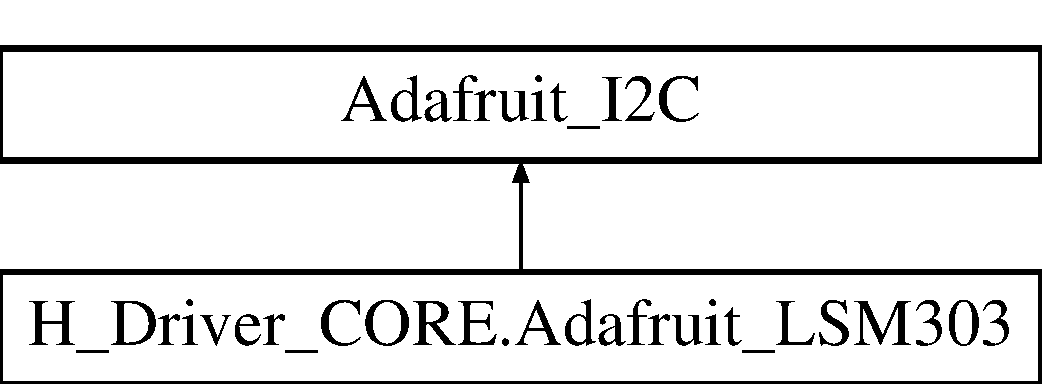
\includegraphics[height=2.000000cm]{classH__Driver__CORE_1_1Adafruit__LSM303}
\end{center}
\end{figure}


\subsection{Detailed Description}
\begin{DoxyVerb}Python library for Adafruit Flora Accelerometer/Compass Sensor (LSM303).
This is pretty much a direct port of the current Arduino library and is
similarly incomplete (e.g. no orientation value returned from read()
method).  This does add optional high resolution mode to accelerometer
though.

Copyright 2013 Adafruit Industries

Version 0.1

Revised October 10, 2014

Revision Author: Isaac DeSouza (IDS LABS)

Copyright 2014 IDS LABS
\end{DoxyVerb}
 

The documentation for this class was generated from the following file\+:\begin{DoxyCompactItemize}
\item 
H\+\_\+\+Driver\+\_\+\+C\+O\+R\+E.\+py\end{DoxyCompactItemize}

\hypertarget{classi2c__lib_1_1i2c__device}{}\section{i2c\+\_\+lib.\+i2c\+\_\+device Class Reference}
\label{classi2c__lib_1_1i2c__device}\index{i2c\+\_\+lib.\+i2c\+\_\+device@{i2c\+\_\+lib.\+i2c\+\_\+device}}
\subsection*{Public Member Functions}
\begin{DoxyCompactItemize}
\item 
\hypertarget{classi2c__lib_1_1i2c__device_afe809fbacb8516d0598b1a2ed9f3bb31}{}def {\bfseries \+\_\+\+\_\+init\+\_\+\+\_\+}\label{classi2c__lib_1_1i2c__device_afe809fbacb8516d0598b1a2ed9f3bb31}

\item 
\hypertarget{classi2c__lib_1_1i2c__device_af32730e22001e6593151d45d5078ec09}{}def {\bfseries write\+\_\+cmd}\label{classi2c__lib_1_1i2c__device_af32730e22001e6593151d45d5078ec09}

\item 
\hypertarget{classi2c__lib_1_1i2c__device_aa3d8df433b3be034a921c1e15eaf0456}{}def {\bfseries write\+\_\+cmd\+\_\+arg}\label{classi2c__lib_1_1i2c__device_aa3d8df433b3be034a921c1e15eaf0456}

\item 
\hypertarget{classi2c__lib_1_1i2c__device_a92b3ddfb4989ba34a4f64170c3196637}{}def {\bfseries write\+\_\+block\+\_\+data}\label{classi2c__lib_1_1i2c__device_a92b3ddfb4989ba34a4f64170c3196637}

\item 
\hypertarget{classi2c__lib_1_1i2c__device_ae3c629c0fef21c4fcfa59972e4bb7b8d}{}def {\bfseries read}\label{classi2c__lib_1_1i2c__device_ae3c629c0fef21c4fcfa59972e4bb7b8d}

\item 
\hypertarget{classi2c__lib_1_1i2c__device_a5848805914a8521974ed1829c2973f06}{}def {\bfseries read\+\_\+data}\label{classi2c__lib_1_1i2c__device_a5848805914a8521974ed1829c2973f06}

\item 
\hypertarget{classi2c__lib_1_1i2c__device_a08fcf0ed296210bb521c3627c633c4a6}{}def {\bfseries read\+\_\+block\+\_\+data}\label{classi2c__lib_1_1i2c__device_a08fcf0ed296210bb521c3627c633c4a6}

\end{DoxyCompactItemize}
\subsection*{Public Attributes}
\begin{DoxyCompactItemize}
\item 
\hypertarget{classi2c__lib_1_1i2c__device_acbed464b8784c5af0ad0cd7c67eee5cf}{}{\bfseries addr}\label{classi2c__lib_1_1i2c__device_acbed464b8784c5af0ad0cd7c67eee5cf}

\item 
\hypertarget{classi2c__lib_1_1i2c__device_a56a3b7c2a48700d69faff94e0af39a93}{}{\bfseries bus}\label{classi2c__lib_1_1i2c__device_a56a3b7c2a48700d69faff94e0af39a93}

\end{DoxyCompactItemize}


The documentation for this class was generated from the following file\+:\begin{DoxyCompactItemize}
\item 
i2c\+\_\+lib.\+py\end{DoxyCompactItemize}

\hypertarget{classH__Driver__CORE_1_1LCD}{}\section{H\+\_\+\+Driver\+\_\+\+C\+O\+R\+E.\+L\+C\+D Class Reference}
\label{classH__Driver__CORE_1_1LCD}\index{H\+\_\+\+Driver\+\_\+\+C\+O\+R\+E.\+L\+C\+D@{H\+\_\+\+Driver\+\_\+\+C\+O\+R\+E.\+L\+C\+D}}


\subsection{Detailed Description}
\begin{DoxyVerb}Driver for 16 Characters 4 line LCD with an I2C interface.

Version 0.1

Revised October 10, 2014

Revision Author: Isaac DeSouza (IDS LABS)

Copyright 2014 IDS LABS
\end{DoxyVerb}
 

The documentation for this class was generated from the following file\+:\begin{DoxyCompactItemize}
\item 
H\+\_\+\+Driver\+\_\+\+C\+O\+R\+E.\+py\end{DoxyCompactItemize}

\hypertarget{classH__Driver__CORE_1_1PCA9865}{}\section{H\+\_\+\+Driver\+\_\+\+C\+O\+R\+E.\+P\+C\+A9865 Class Reference}
\label{classH__Driver__CORE_1_1PCA9865}\index{H\+\_\+\+Driver\+\_\+\+C\+O\+R\+E.\+P\+C\+A9865@{H\+\_\+\+Driver\+\_\+\+C\+O\+R\+E.\+P\+C\+A9865}}
\subsection*{Public Member Functions}
\begin{DoxyCompactItemize}
\item 
def \hyperlink{classH__Driver__CORE_1_1PCA9865_ad55ae8ab9ca6bd8381edde60fcf886c1}{\+\_\+\+\_\+init\+\_\+\+\_\+}
\item 
def \hyperlink{classH__Driver__CORE_1_1PCA9865_a746e1e3746dec4f182484e4dddeea50a}{set\+Freq}
\item 
def \hyperlink{classH__Driver__CORE_1_1PCA9865_a5724a0ad0d377db94c552640986a8cba}{\+\_\+\+\_\+calc\+\_\+prescale\+\_\+\+\_\+}
\end{DoxyCompactItemize}
\subsection*{Public Attributes}
\begin{DoxyCompactItemize}
\item 
\hypertarget{classH__Driver__CORE_1_1PCA9865_ac22b8744829ffb2e6eda8bdeea34e398}{}{\bfseries i2c}\label{classH__Driver__CORE_1_1PCA9865_ac22b8744829ffb2e6eda8bdeea34e398}

\end{DoxyCompactItemize}
\subsection*{Static Public Attributes}
\begin{DoxyCompactItemize}
\item 
\hypertarget{classH__Driver__CORE_1_1PCA9865_a2318d8d4faca392d39776aed8ab66ebc}{}int {\bfseries F\+R\+E\+Q\+\_\+\+M\+I\+N} = 50\label{classH__Driver__CORE_1_1PCA9865_a2318d8d4faca392d39776aed8ab66ebc}

\item 
\hypertarget{classH__Driver__CORE_1_1PCA9865_ae8e739fb7135848ec137f39bf49bb458}{}int {\bfseries F\+R\+E\+Q\+\_\+\+M\+A\+X} = 300\label{classH__Driver__CORE_1_1PCA9865_ae8e739fb7135848ec137f39bf49bb458}

\end{DoxyCompactItemize}


\subsection{Constructor \& Destructor Documentation}
\hypertarget{classH__Driver__CORE_1_1PCA9865_ad55ae8ab9ca6bd8381edde60fcf886c1}{}\index{H\+\_\+\+Driver\+\_\+\+C\+O\+R\+E\+::\+P\+C\+A9865@{H\+\_\+\+Driver\+\_\+\+C\+O\+R\+E\+::\+P\+C\+A9865}!\+\_\+\+\_\+init\+\_\+\+\_\+@{\+\_\+\+\_\+init\+\_\+\+\_\+}}
\index{\+\_\+\+\_\+init\+\_\+\+\_\+@{\+\_\+\+\_\+init\+\_\+\+\_\+}!H\+\_\+\+Driver\+\_\+\+C\+O\+R\+E\+::\+P\+C\+A9865@{H\+\_\+\+Driver\+\_\+\+C\+O\+R\+E\+::\+P\+C\+A9865}}
\subsubsection[{\+\_\+\+\_\+init\+\_\+\+\_\+}]{\setlength{\rightskip}{0pt plus 5cm}def H\+\_\+\+Driver\+\_\+\+C\+O\+R\+E.\+P\+C\+A9865.\+\_\+\+\_\+init\+\_\+\+\_\+ (
\begin{DoxyParamCaption}
\item[{}]{self, }
\item[{}]{busnum = {\ttfamily -\/1}, }
\item[{}]{debug = {\ttfamily False}, }
\item[{}]{port}
\end{DoxyParamCaption}
)}\label{classH__Driver__CORE_1_1PCA9865_ad55ae8ab9ca6bd8381edde60fcf886c1}
\begin{DoxyVerb}When creating driver objects the port for the device must be specified. Ports are integers values from 1 - 2. Returns nothing.
\end{DoxyVerb}
 

\subsection{Member Function Documentation}
\hypertarget{classH__Driver__CORE_1_1PCA9865_a5724a0ad0d377db94c552640986a8cba}{}\index{H\+\_\+\+Driver\+\_\+\+C\+O\+R\+E\+::\+P\+C\+A9865@{H\+\_\+\+Driver\+\_\+\+C\+O\+R\+E\+::\+P\+C\+A9865}!\+\_\+\+\_\+calc\+\_\+prescale\+\_\+\+\_\+@{\+\_\+\+\_\+calc\+\_\+prescale\+\_\+\+\_\+}}
\index{\+\_\+\+\_\+calc\+\_\+prescale\+\_\+\+\_\+@{\+\_\+\+\_\+calc\+\_\+prescale\+\_\+\+\_\+}!H\+\_\+\+Driver\+\_\+\+C\+O\+R\+E\+::\+P\+C\+A9865@{H\+\_\+\+Driver\+\_\+\+C\+O\+R\+E\+::\+P\+C\+A9865}}
\subsubsection[{\+\_\+\+\_\+calc\+\_\+prescale\+\_\+\+\_\+}]{\setlength{\rightskip}{0pt plus 5cm}def H\+\_\+\+Driver\+\_\+\+C\+O\+R\+E.\+P\+C\+A9865.\+\_\+\+\_\+calc\+\_\+prescale\+\_\+\+\_\+ (
\begin{DoxyParamCaption}
\item[{}]{self, }
\item[{}]{freq}
\end{DoxyParamCaption}
)}\label{classH__Driver__CORE_1_1PCA9865_a5724a0ad0d377db94c552640986a8cba}
\begin{DoxyVerb}Converts the input frequency into the appropriate values for the PCA9865 driver. See PCA9865 datasheet for more information.
\end{DoxyVerb}
 \hypertarget{classH__Driver__CORE_1_1PCA9865_a746e1e3746dec4f182484e4dddeea50a}{}\index{H\+\_\+\+Driver\+\_\+\+C\+O\+R\+E\+::\+P\+C\+A9865@{H\+\_\+\+Driver\+\_\+\+C\+O\+R\+E\+::\+P\+C\+A9865}!set\+Freq@{set\+Freq}}
\index{set\+Freq@{set\+Freq}!H\+\_\+\+Driver\+\_\+\+C\+O\+R\+E\+::\+P\+C\+A9865@{H\+\_\+\+Driver\+\_\+\+C\+O\+R\+E\+::\+P\+C\+A9865}}
\subsubsection[{set\+Freq}]{\setlength{\rightskip}{0pt plus 5cm}def H\+\_\+\+Driver\+\_\+\+C\+O\+R\+E.\+P\+C\+A9865.\+set\+Freq (
\begin{DoxyParamCaption}
\item[{}]{self, }
\item[{}]{freq}
\end{DoxyParamCaption}
)}\label{classH__Driver__CORE_1_1PCA9865_a746e1e3746dec4f182484e4dddeea50a}
\begin{DoxyVerb}Sets the oscillator frequency for the PCA9865 driver. Frequency values from 50 to 300 are allowed.
\end{DoxyVerb}
 

The documentation for this class was generated from the following file\+:\begin{DoxyCompactItemize}
\item 
H\+\_\+\+Driver\+\_\+\+C\+O\+R\+E.\+py\end{DoxyCompactItemize}

%--- End generated contents ---

% Index
\backmatter
\newpage
\phantomsection
\clearemptydoublepage
\addcontentsline{toc}{chapter}{Index}
\printindex

\end{document}
